\documentclass[aspectratio=169]{beamer}

\usetheme{Madrid}
\usecolortheme{default}
\setbeamertemplate{navigation symbols}{}

\usepackage[utf8]{inputenc}
\usepackage[T1]{fontenc}
\usepackage{lmodern}
\usepackage{graphicx}
\usepackage{booktabs}
\usepackage{array}
\usepackage{xcolor}
\usepackage{tikz}

\definecolor{accent}{RGB}{30,72,138}
\definecolor{soft}{RGB}{241,245,249}
\definecolor{good}{RGB}{22,101,52}
\definecolor{warn}{RGB}{180,83,9}

\setbeamercolor{title}{fg=accent}
\setbeamercolor{frametitle}{fg=accent}
\setbeamercolor{block title}{bg=accent!12,fg=black}
\setbeamercolor{block body}{bg=soft,fg=black}

\title{Hesaplamali Anlambilim 2. Odev}
\subtitle{LLM Trajectory Analysis}
\author{Hamza Vedat Cengiz}
\date{Nisan 2026}

\begin{document}

\begin{frame}
  \titlepage
\end{frame}

\begin{frame}{Problem}
  \begin{block}{Odevin ana fikri}
    Dil modelinin sadece \textbf{urettigi metne} degil, metni uretirken iceride olusan
    \textbf{temsil hareketine} bakiyoruz.
  \end{block}

  \vspace{0.4em}
  \begin{itemize}
    \item Iki farkli causal language model secildi.
    \item Her model icin en az 1000 trajectory toplandi.
    \item Her trajectory en az 50 tokenlik uretimden olustu.
    \item Trajectory'lerden ozellik cikarilip iki tahmin gorevi kuruldu.
  \end{itemize}
\end{frame}

\begin{frame}{Temel Kavramlar}
  \begin{columns}[T]
    \column{0.48\textwidth}
    \begin{block}{Token}
      Modelin metni islerken kullandigi parcadir. Her zaman tam kelime olmak zorunda degildir.
    \end{block}

    \begin{block}{Hidden state}
      Modelin o andaki ic sayisal durumu. Bir sonraki token seciminden hemen onceki vektor temsilidir.
    \end{block}

    \column{0.48\textwidth}
    \begin{block}{Trajectory}
      Uretim sirasinda her adimda son-token hidden state'i kaydedilirse zaman icinde bir vektor dizisi olusur.
    \end{block}

    \begin{block}{Yazilimci benzetmesi}
      Bir servisin loglarini degil, runtime ic durumunun zaman serisini inceliyoruz.
    \end{block}
  \end{columns}
\end{frame}

\begin{frame}{Kullandigim Modeller ve Veri}
  \begin{itemize}
    \item Modeller: \texttt{gpt2} ve \texttt{EleutherAI/pythia-70m}
    \item Toplam trajectory sayisi: \textbf{2000}
    \item Model basina trajectory: \textbf{1000}
    \item Kategori sayisi: \textbf{5}
    \item Kategoriler: History, Science, Technology, Art, Sports
    \item Uretim uzunlugu: \textbf{50 token}
  \end{itemize}

  \vspace{0.5em}
  \begin{block}{Neden iki gorev kuruldu?}
    Trajectory ozellikleri model kimligini ve prompt kategorisini ne kadar tasiyor, bunu gormek icin.
  \end{block}
\end{frame}

\begin{frame}{Pipeline}
  \begin{enumerate}
    \item Prompt verildi.
    \item Model token token uretim yapti.
    \item Her adimda son-layer son-token hidden state kaydedildi.
    \item Her ornek icin bir trajectory dosyasi olustu.
    \item Trajectory'lerden geometric ve normalized/scale-invariant feature'lar cikarildi.
    \item Siniflandirma deneyleri calistirildi.
    \item Sonuclar raporlandi ve gorsellestirildi.
  \end{enumerate}

  \vspace{0.4em}
  \begin{block}{Kod dosyalari}
    \texttt{collect\_data.py}, \texttt{extract\_features.py}, \texttt{predict.py}, \texttt{visualize.py}
  \end{block}
\end{frame}

\begin{frame}{Tahmin Gorevleri}
  \begin{columns}[T]
    \column{0.48\textwidth}
    \begin{block}{Gorev 1: Model identity}
      Soru: Bu trajectory hangi modelden geldi?
      \begin{itemize}
        \item siniflar: GPT-2 vs Pythia-70M
        \item amac: trajectory model imzasi tasiyor mu?
      \end{itemize}
    \end{block}

    \column{0.48\textwidth}
    \begin{block}{Gorev 2: Prompt category}
      Soru: Bu trajectory hangi kategoriye ait?
      \begin{itemize}
        \item 5 kategori
        \item grouped split kullanildi
        \item prompt template leakage azaltildi
      \end{itemize}
    \end{block}
  \end{columns}
\end{frame}

\begin{frame}{Feature Sets}
  \begin{block}{Kullanilan feature aileleri}
    \begin{itemize}
      \item \textbf{Raw geometric}: adimlar arasi mesafe, yol uzunlugu, linearity
      \item \textbf{Normalized geometric}: olcek etkisini azaltan geometric ozetler
      \item \textbf{Scale-invariant}: goreli degisim ve donus davranisini ozetleyen feature'lar
    \end{itemize}
  \end{block}

  \vspace{0.5em}
  \begin{itemize}
    \item Raw sonuclar sadece baseline olarak kullanildi.
    \item Ana yorum normalized + scale-invariant feature'lar uzerinden yapildi.
    \item Category prediction icin grouped split coverage kontrolu eklendi.
  \end{itemize}
\end{frame}

\begin{frame}{Gorsellestirme 1: Model Bazli Trajectory Panelleri}
  \centering
  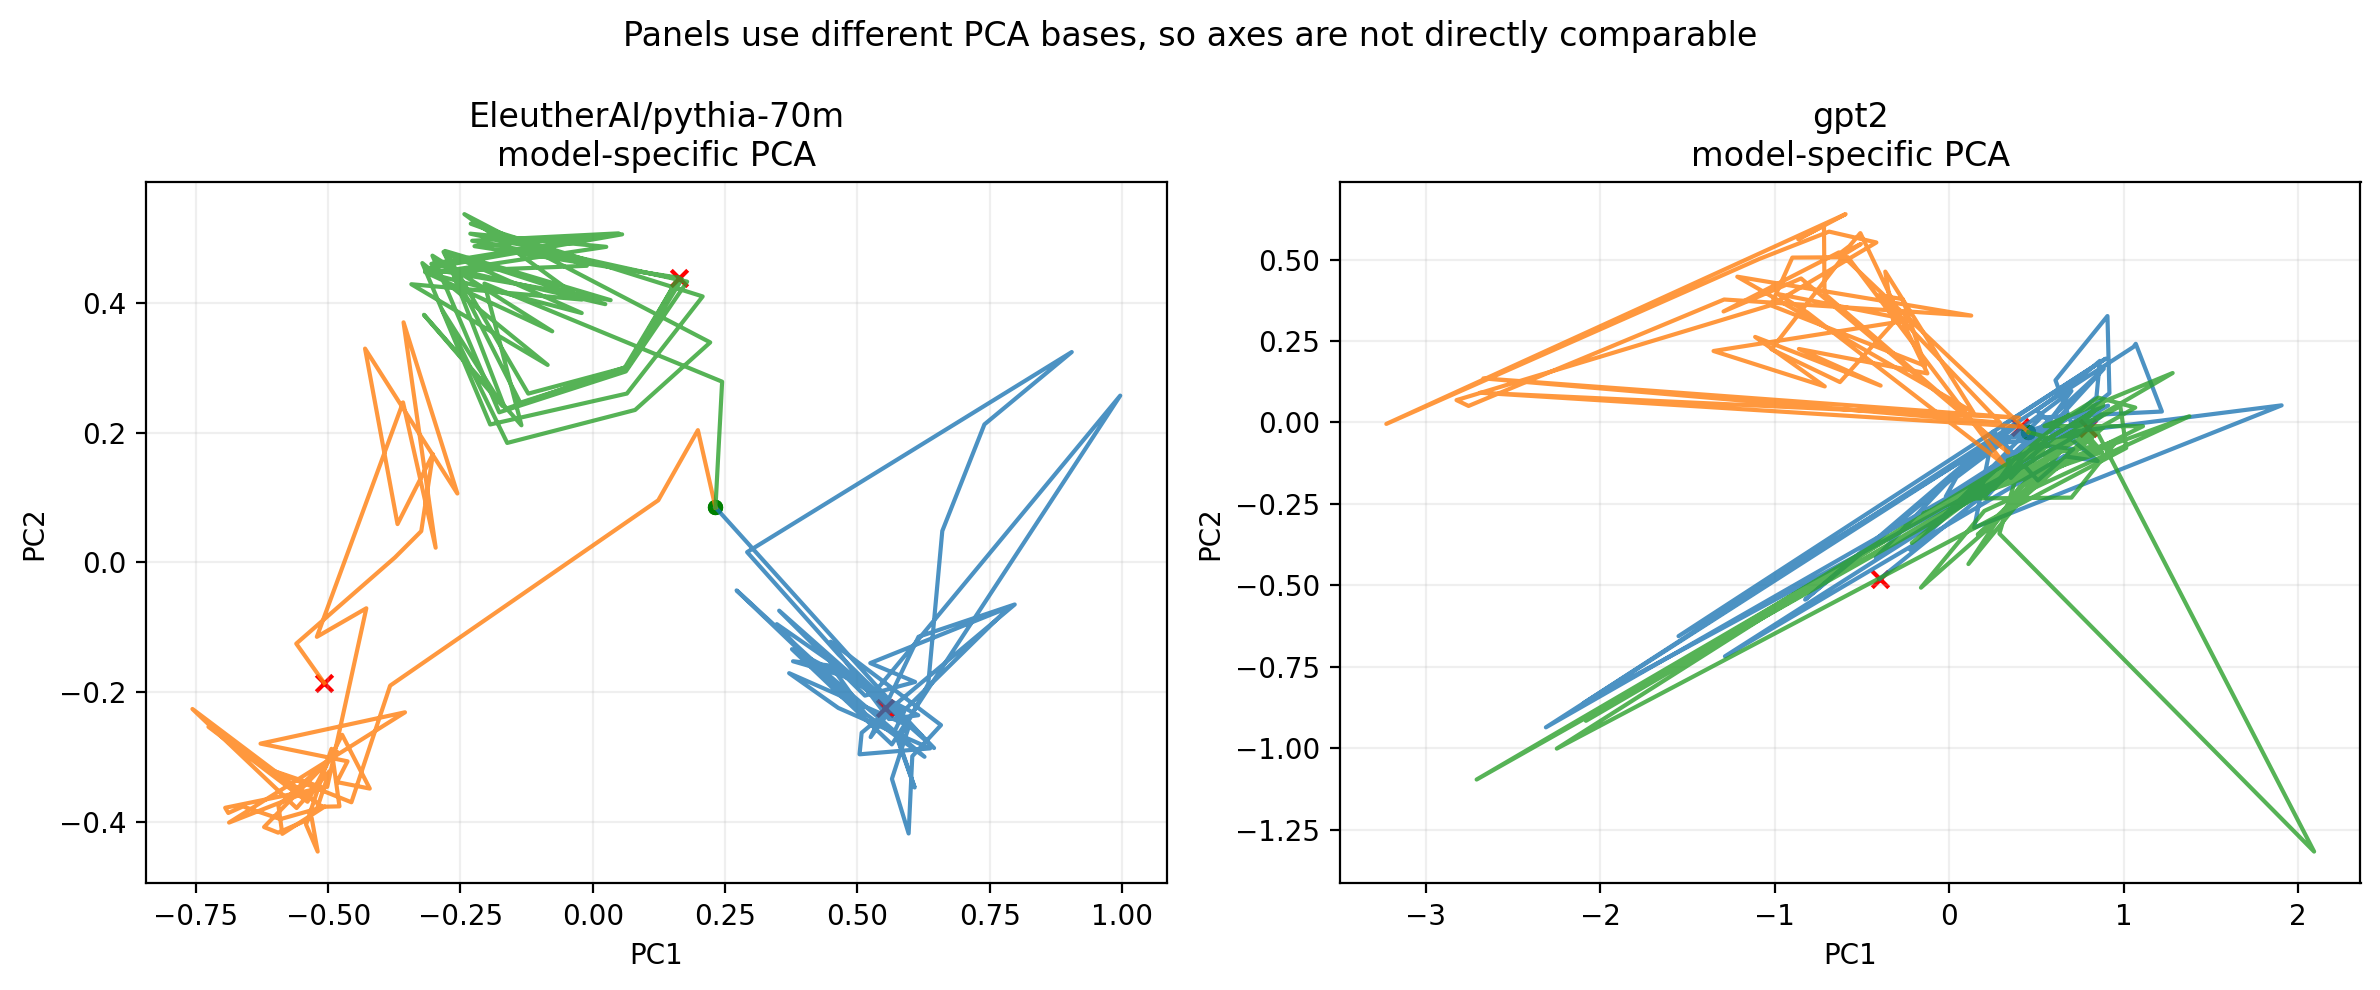
\includegraphics[width=\linewidth,height=0.68\textheight,keepaspectratio]{runs/hw2_full_seed42/plots/trajectories_model_specific_pca.png}

  \vspace{0.4em}
  {\footnotesize Her panel model-ozel PCA bazinda cizildi. Panellerin eksenleri birebir karsilastirilmaz; amac her modelin kendi icindeki trajectory davranisini gormektir.}
\end{frame}

\begin{frame}{Gorsellestirme 2: Ortak Feature Space}
  \centering
  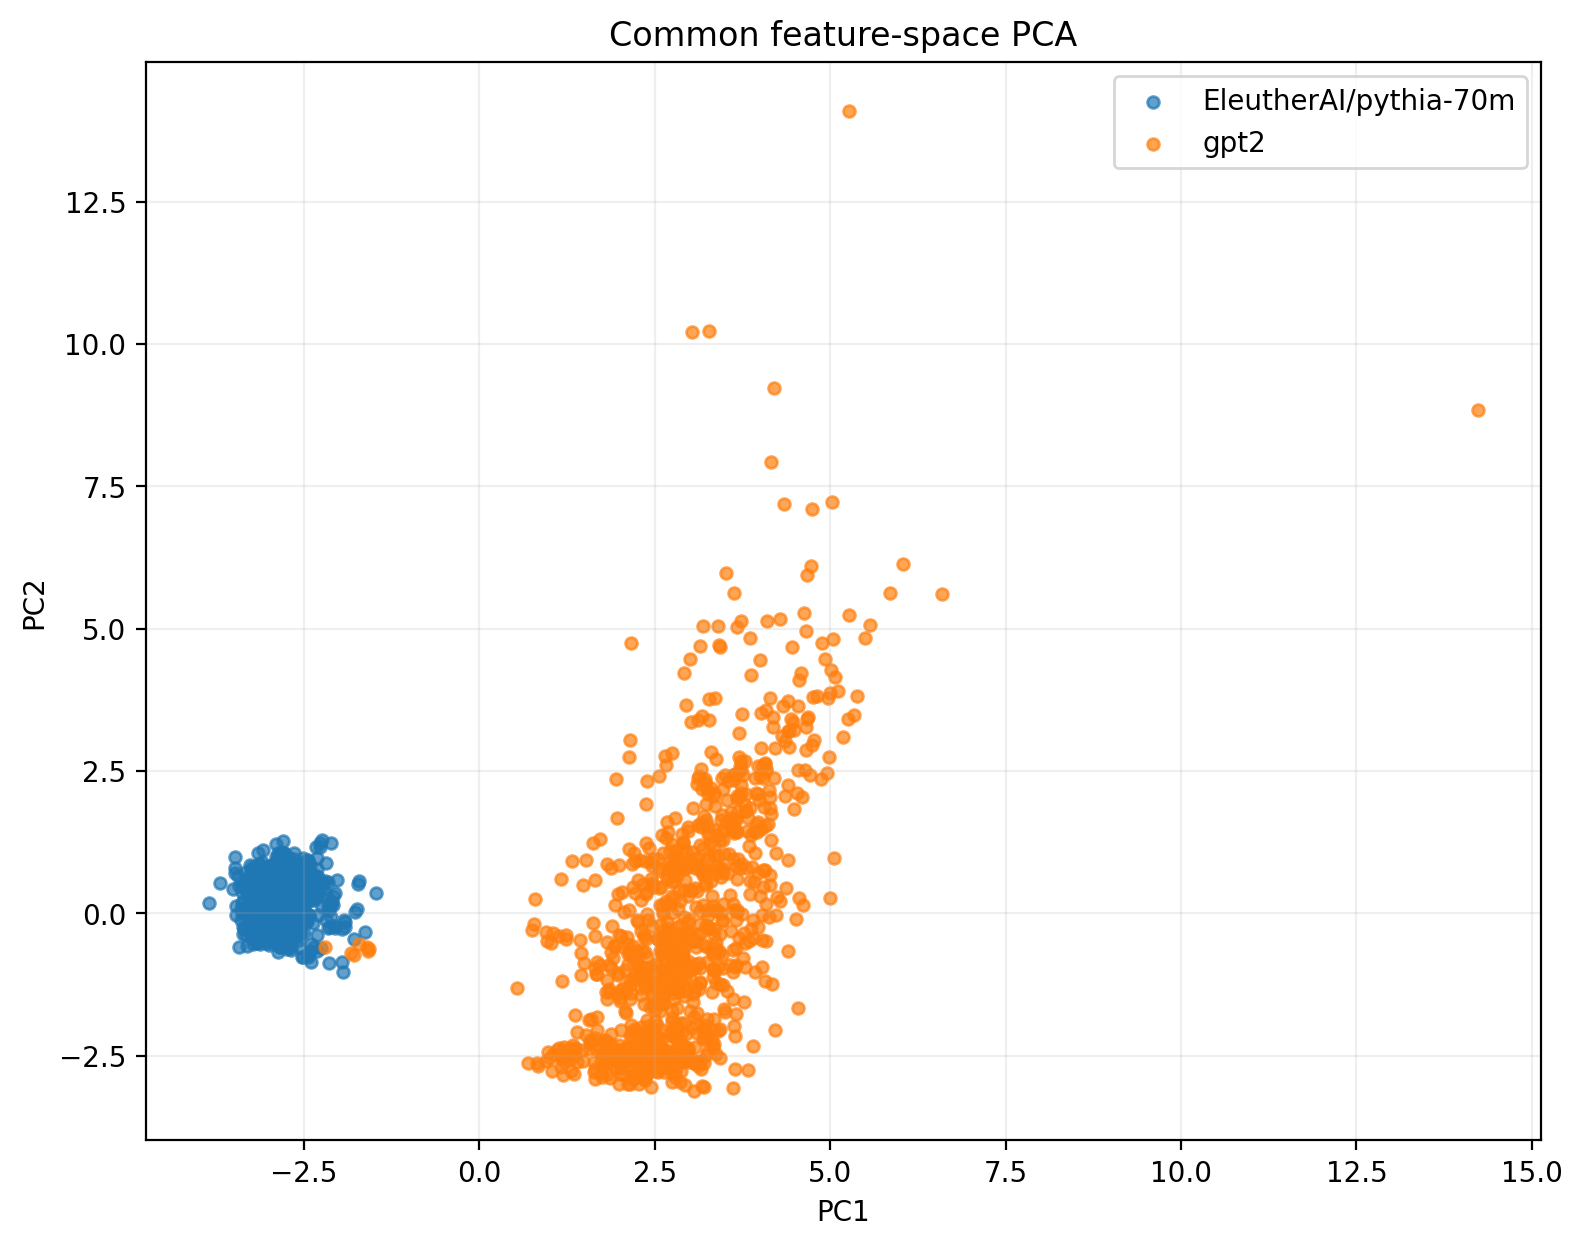
\includegraphics[width=\linewidth,height=0.68\textheight,keepaspectratio]{runs/hw2_full_seed42/plots/common_feature_space_pca.png}

  \vspace{0.4em}
  {\footnotesize Bu PCA ortak feature uzayinda cizildi, bu nedenle modeller arasi dagilim farki ayni koordinat sisteminde okunabilir.}
\end{frame}

\begin{frame}{Sayisal Sonuclar}
  \small
  \begin{table}
    \centering
    \begin{tabular}{>{\raggedright\arraybackslash}p{4.3cm}cc}
      \toprule
      Gorev ve setting & Random Forest & Logistic Regression \\
      \midrule
      Model identity (raw) & 1.0000 & 1.0000 \\
      Model identity (normalized main) & \textbf{0.9975} & \textbf{1.0000} \\
      Category (grouped, raw) & 0.2405 & 0.2095 \\
      Category (grouped, normalized main) & \textbf{0.2143} & \textbf{0.2071} \\
      \bottomrule
    \end{tabular}
  \end{table}

  \vspace{0.5em}
  \begin{block}{Coverage kontrolu}
    Grouped split coverage satisfied = \textbf{True}
  \end{block}
\end{frame}

\begin{frame}{Yorum}
  \begin{itemize}
    \item Model identity sonucu neredeyse kusursuz: trajectory'ler model bazli guclu bir imza tasiyor.
    \item Category sonucu dusuk: mevcut feature set ile kategori bilgisi belirgin sekilde ayrismiyor.
    \item 5 kategori oldugu icin category task'ta sonuc neredeyse sans seviyesine yakin.
    \item Bu, trajectory'lerin once model dinamikleri tarafindan sekillendigini dusundurebilir.
  \end{itemize}

  \vspace{0.5em}
  \begin{block}{Kisa yorum}
    Modelin \textbf{hangi model oldugu} trajectory'den cok iyi anlasiliyor; ancak
    \textbf{hangi konu kategorisinden geldigi} ayni gucle anlasilmiyor.
  \end{block}
\end{frame}

\begin{frame}{Metodolojik Duzeltmeler}
  \begin{itemize}
    \item Reproducible run klasorleri ve \texttt{run\_config.json}
    \item Gercek seed kullanimi ve reproducibility check
    \item Prompt-template leakage azaltmak icin grouped split
    \item Coverage saglanmazsa error/warn politikasi
    \item Raw ve normalized feature sonuclarinin ayrilmasi
    \item Analitik olarak gecerli gorsellestirme stratejisi
  \end{itemize}
\end{frame}

\begin{frame}{Sinirliliklar ve Gelecek Is}
  \begin{itemize}
    \item Sadece iki kucuk model kullanildi.
    \item Feature set daha zenginlestirilebilir.
    \item Farkli model aileleri ve daha buyuk modeller denenebilir.
    \item Kategori yerine farkli hedefler test edilebilir:
      \begin{itemize}
        \item tekrar davranisi
        \item metin kalitesi
        \item entropy veya sampling davranisi
      \end{itemize}
  \end{itemize}
\end{frame}

\begin{frame}{Sonuc}
  \begin{block}{Ana cikti}
    Bu proje, dil modellerinin metin uretirken olusan ic temsil hareketlerinin
    anlamli sekilde analiz edilebilecegini gosteriyor.
  \end{block}

  \vspace{0.5em}
  \begin{itemize}
    \item Trajectory'ler model farkini guclu sekilde tasiyor.
    \item Ayni feature'lar kategori bilgisini guclu tasimiyor.
    \item Yani bu calisma daha cok \textbf{model behavior analysis} olarak okunmali.
  \end{itemize}

  \vspace{0.8em}
  \centering
  {\Large Tesekkurler}
\end{frame}

\end{document}
